Supersymmetry (SUSY)~\cite{SUSYPrimer} is an extension to the standard model that can explain some of the open problems in physics such as
a solution the hierarchy problem as well as providing potential candidates for dark matter.
Searches for SUSY are performed by the CMS collaboration in a variety of final states,
including searching for processes with leptons (e or $\mu$) in the final state.
Simplified models~\cite{sms} are used to interpret results of these searches, where two examples are shown in figure~\ref{fig:SMS}.
On the left is a diagram of a gauge mediated SUSY breaking (GMSB) model with a massless gravitino as the lightest SUSY particle (LSP).
In this model, gluinos are pair produced, and each decays to a pair of quarks and a neutralino, which subsequently decays to a Z boson and a gravitino.
Another model showing direct stop production with one of the stops eventually
decaying to a top that decays leptonically is shown on the right.
The results presented in these proceedings focus on direct squark and gluino production.
In all of the following results, no significant deviation from the SM was observed,
and limits are set on the upper limit of the cross section of simplified models at the 95\% level using the CLs method~\cite{Junk:1999kv,Read:2002hq}.

\begin{figure}[!htb]
\begin{center}
\begin{tabular}{cc}
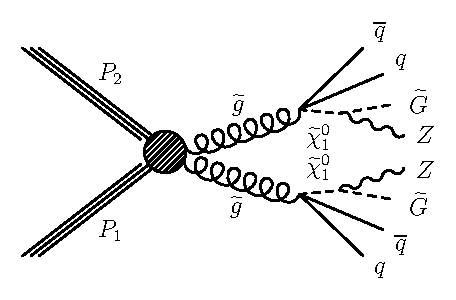
\includegraphics[width=0.4\textwidth]{intro/Feynman_graph_T5ZZgmsb.pdf} &
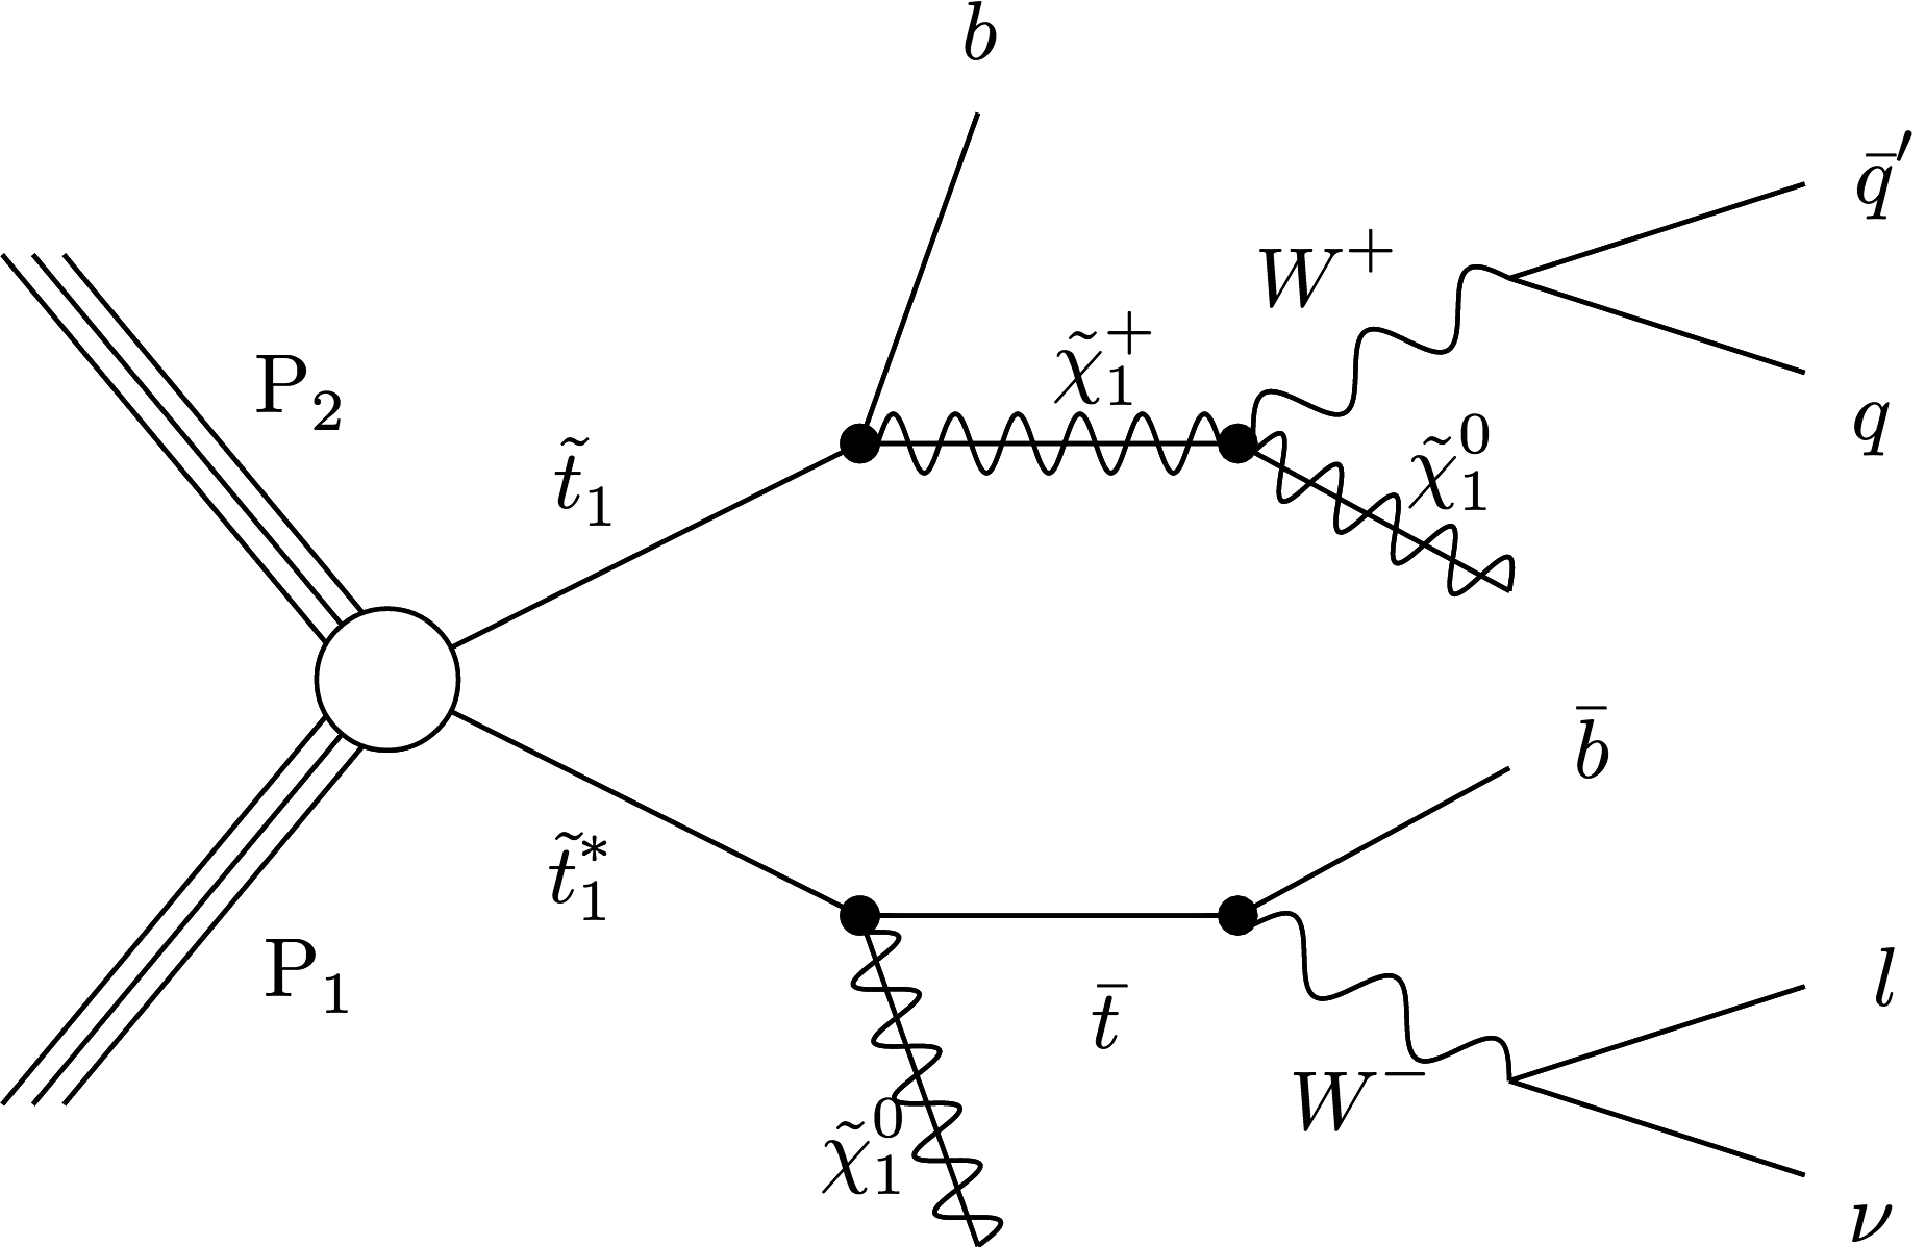
\includegraphics[width=0.4\textwidth]{intro/T2tt.pdf}
\end{tabular}
\caption{
\label{fig:SMS}
Diagrams showing different SUSY processes which may contain leptons in the final state are shown in this figure.
On the left, gravitinos are pair-produced, where each eventually decays to a Z boson, two quarks, and a gravitino.
On the right, stops are pair-produced, where one leg eventually decays to a top and a neutralino where the top decays leptonically.
}
\end{center}
\end{figure}

The SUSY analyses performed by CMS target a large range of topologies with varying
visible energy
(\HT, \MJ), 
invisible energy (\MET, \MT, \MTtwo, \dphiwl, \LT),
jet multiplicity (\njets)
and flavor content (\nbtags).
The analyses are grouped by the number of leptons in the final state,
and for analyses with at least two leptons,
they are categorized according to the charge of the two leptons with the highest \pt
in same-sign, or opposite-sign final states.
